% !TeX program = xelatex
\documentclass[11pt,a4paper,fontset=fandol]{ctexart}

% ============================ 1. 基础页面设置 ================================
\usepackage{geometry}
\geometry{left=2.5cm, right=2.5cm, top=2.5cm, bottom=2.5cm}

% ============================ 2. 数学基础包与标准定理 ========================
\usepackage{amsmath, amssymb, amsthm}
\usepackage{mathtools}
\usepackage{bm}                       % 向量/矩阵加粗
\allowdisplaybreaks                   % 长公式跨页

% 标准学术定理环境
\newtheorem{theorem}{定理}[section]
\newtheorem{lemma}[theorem]{引理}
\newtheorem{property}[theorem]{性质}
\newtheorem{corollary}[theorem]{推论}
\newtheorem{example}{例题}[section]

\theoremstyle{remark}
\newtheorem{remark}{注}[section]

% ============================ 3. 字体设置 ====================================
\usepackage{newtxtext}               % 英文 Times 系列
\usepackage{newtxmath}               % 数学公式 Times 系列

% ============================ 4. 独立定义环境 ================================
\usepackage[most]{tcolorbox}

% 定义环境：学术极简浅灰底+细边框
\newtcbtheorem[number within=section]{definition}{定义}{
    enhanced,
    boxrule=0.5pt,
    arc=0pt,
    colback=gray!4!white,
    colframe=black!80,
    fonttitle=\bfseries\sffamily,
    coltitle=black,
    attach boxed title to top left={yshift=-2mm, xshift=2mm},
    boxed title style={boxrule=0pt, colframe=white, colback=white},
    separator sign={\ },
    description font=\normalfont
}{def}

% ============================ 5. 图表、列表与绘图 ============================
\usepackage{booktabs}
\usepackage{graphicx}
\usepackage{enumitem}
\setlist{nosep, leftmargin=2em}

\usepackage{caption}
\captionsetup{font=small, labelfont=bf, justification=centering}

\usepackage{tikz}
\usetikzlibrary{arrows.meta, decorations.markings, calc, patterns}

% ============================ 6. 超链接设置 ==================================
\usepackage{hyperref}
\usepackage{cleveref}
\hypersetup{
    colorlinks=true,
    linkcolor=black,
    citecolor=black,
    urlcolor=black
}

% ============================ 7. 章节格式 ====================================
\ctexset{
    section/name={,},
    section/number=\arabic{section},
    section/format=\Large\bfseries,
    subsection/number=\arabic{section}.\arabic{subsection},
    subsection/format=\large\bfseries,
    subsubsection/number=\arabic{section}.\arabic{subsection}.\arabic{subsubsection},
    subsubsection/format=\normalsize\bfseries
}

\renewcommand{\baselinestretch}{1.15}
\setlength{\parskip}{0.3em}
\setlength{\parindent}{2em}

% ============================ 8. 页眉页脚 ====================================
\usepackage{fancyhdr}
\pagestyle{fancy}
\fancyhf{}
\fancyhead[L]{\small 大学物理}
\fancyhead[R]{\small \leftmark}
\fancyfoot[C]{\small\thepage}
\renewcommand{\headrulewidth}{0.4pt}

% ============================ 9. 正文开始 ====================================
\begin{document}

\section{静电场}

\subsection{电荷守恒定律与库仑定律}

\begin{definition}{电荷守恒定律}{charge_conservation}
在一个与外界没有电荷交换的孤立系统中，无论发生何种物理或化学过程，系统内所有正、负电荷的代数和始终保持不变。电荷不能被凭空创造，也不能被凭空消灭。
\end{definition}

\begin{definition}{库仑定律与点电荷}{coulomb_law}
真空中有两个静止的点电荷 $q_1$ 和 $q_2$，它们之间的静电相互作用力大小与电荷量乘积成正比，与它们之间距离的二次方成反比；作用力的方向沿着两者的连线。真空中库仑力数学表达式为：
\begin{equation}
    \bm{F}_{12} = \frac{1}{4\pi\varepsilon_0}\frac{q_1 q_2}{r_{12}^2}\hat{\bm{r}}_{12}
\end{equation}
其中 $\varepsilon_0 \approx 8.854 \times 10^{-12}\,\mathrm{F/m}$ 为真空介电常数，$\hat{\bm{r}}_{12}$ 是由 $q_1$ 指向 $q_2$ 的单位矢量。
\end{definition}

\begin{property}[静电力叠加原理]
点电荷系中，任一点电荷受到的合静电力等于其它各电荷单独存在时对该点电荷作用力的矢量和，即 $\bm{F} = \sum_{i} \bm{F}_i$。
\end{property}

\subsection{电场强度与场强叠加原理}

\begin{definition}{电场强度}{electric_field}
电场强度 $\bm{E}$ 是描述电场力的性质的物理量。其定义为单位正试验电荷 $q_0$ 放在电场中某点所受到的电场力 $\bm{F}$：
\begin{equation}
    \bm{E} = \lim_{q_0 \to 0} \frac{\bm{F}}{q_0}
\end{equation}
点电荷 $q$ 在空间距离 $r$ 处产生的场强为：$\bm{E} = \frac{q}{4\pi\varepsilon_0 r^2}\hat{\bm{r}}$。
\end{definition}

对于连续带电体，电场强度通过微元积分求解：
\begin{equation}
    \bm{E} = \int \mathrm{d}\bm{E} = \frac{1}{4\pi\varepsilon_0} \int \frac{\mathrm{d}q}{r^2}\hat{\bm{r}}
\end{equation}
式中 $\mathrm{d}q$ 分别由线电荷密度 $\lambda\,\mathrm{d}l$、面电荷密度 $\sigma\,\mathrm{d}S$ 或体电荷密度 $\rho\,\mathrm{d}V$ 给出。

\subsection{静电场的高斯定理}

\begin{definition}{电通量}{electric_flux}
穿过电场中某一有向曲面 $S$ 的电场线条数称为电通量，用 $\Phi_e$ 表示：
\begin{equation}
    \Phi_e = \iint_S \bm{E} \cdot \mathrm{d}\bm{S} = \iint_S E \cos\theta\,\mathrm{d}S
\end{equation}
对于闭合曲面，面元矢量 $\mathrm{d}\bm{S}$ 约定一律指向闭合面的外法线方向。
\end{definition}

\begin{theorem}[静电场的高斯定理]
在真空中，穿过任意闭合曲面 $S$（称为高斯面）的电场强度通量 $\Phi_e$，等于该闭合曲面所包围的电荷电量代数和除以真空介电常数 $\varepsilon_0$，与闭合曲面外的电荷无关：
\begin{equation}
    \oint_S \bm{E} \cdot \mathrm{d}\bm{S} = \frac{1}{\varepsilon_0}\sum q_{\text{内}}
\end{equation}
其微分形式表述为：$\nabla \cdot \bm{E} = \frac{\rho}{\varepsilon_0}$。这表明静电场是有源场，电荷是静电场的源。
\end{theorem}

\begin{remark}[利用高斯定理求解场强的关键步骤]
高斯定理恒成立，但仅在电荷分布具有高度对称性时方可直接求解 $\bm{E}$：
\begin{enumerate}
    \item \textbf{对称性分析}：根据电荷空间分布判断场强方向的分布特征（球对称、轴对称或平面对称）。
    \item \textbf{选取高斯面}：选取的闭合面必须使待求场强的点落在面上，且高斯面各部分满足 $\bm{E} \perp \mathrm{d}\bm{S}$（通量为 0）或 $\bm{E} \parallel \mathrm{d}\bm{S}$ 且 $|\bm{E}| = \text{常数}$（通量可提至积分号外化为 $E \cdot S$）。
    \item \textbf{计算电量与通量}：分别求出 $\oint_S \bm{E}\cdot\mathrm{d}\bm{S}$ 与面内包围的总电荷量 $\sum q_{\text{内}}$。
    \item \textbf{列式求解}：令 $\oint \bm{E}\cdot\mathrm{d}\bm{S} = \frac{1}{\varepsilon_0}\sum q_{\text{内}}$，解得场强分布大小并标出方向。
\end{enumerate}
\end{remark}

% ------------------------- 球对称例题 -------------------------
\begin{example}[球对称：同心带电导体球与球壳]
如图所示，一半径为 $R_1$ 的导体球带有电量 $q_1$，其外同心地放置一内半径为 $R_2$、外半径为 $R_3$ 的带电导体球壳，球壳带有总电荷 $q_2$。求各区域的电场强度 $\bm{E}$ 分布。

\begin{center}
\begin{tikzpicture}[scale=1.0]
    % 导体球
    \fill[ball color=gray!30] (0,0) circle (1.0);
    \draw[thick] (0,0) circle (1.0);
    % 导体球壳
    \fill[even odd rule, fill=gray!20] (0,0) circle (2.2) (0,0) circle (1.6);
    \draw[thick] (0,0) circle (1.6);
    \draw[thick] (0,0) circle (2.2);
    % 高斯面示例 (虚线)
    \draw[dashed, red, thick] (0,0) circle (1.3);
    \node[red, right] at (0.9, 0.9) {$S_{\text{高斯}}$};
    % 标尺与半径
    \draw[-{Stealth}] (0,0) -- (45:1.0) node[midway, above left] {\footnotesize $R_1$};
    \draw[-{Stealth}] (0,0) -- (-30:1.6) node[midway, below] {\footnotesize $R_2$};
    \draw[-{Stealth}] (0,0) -- (120:2.2) node[midway, left] {\footnotesize $R_3$};
    \fill (0,0) circle (1.5pt) node[below] {$O$};
    \node at (0, 0.5) {$q_1$};
    \node at (0, 1.9) {$q_2$};
\end{tikzpicture}
\captionof{figure}{同心球壳系统的几何结构与同心高斯球面}
\end{center}

\textbf{解}：
由电荷分布的球对称性，全空间的电场强度方向必沿径向，大小仅取决于径向距离 $r$，即 $\bm{E} = E(r)\hat{\bm{r}}$。取以 $O$ 为中心、半径为 $r$ 的同心球面为高斯面，高斯面积分为：
\begin{equation*}
    \oint_S \bm{E} \cdot \mathrm{d}\bm{S} = E(r) \cdot 4\pi r^2
\end{equation*}
分区域计算包围的净电荷量：
\begin{enumerate}
    \item 当 $r < R_1$ 时，高斯面内处于内部导体球内，$\sum q_{\text{内}} = 0 \implies E_1 = 0$。
    \item 当 $R_1 < r < R_2$ 时，高斯面仅包围导体球，$\sum q_{\text{内}} = q_1$：
    \begin{equation*}
        E(r) \cdot 4\pi r^2 = \frac{q_1}{\varepsilon_0} \implies E_2(r) = \frac{q_1}{4\pi\varepsilon_0 r^2}
    \end{equation*}
    \item 当 $R_2 < r < R_3$ 时，高斯面处于球壳导体内，静电平衡下场强处处为零，即 $E_3 = 0$。
    \item 当 $r > R_3$ 时，高斯面包围了球和球壳的全部电荷，$\sum q_{\text{内}} = q_1 + q_2$：
    \begin{equation*}
        E(r) \cdot 4\pi r^2 = \frac{q_1 + q_2}{\varepsilon_0} \implies E_4(r) = \frac{q_1 + q_2}{4\pi\varepsilon_0 r^2}
    \end{equation*}
\end{enumerate}
\end{example}

% ------------------------- 轴对称例题 -------------------------
\begin{example}[轴对称：无限长均匀带电圆柱面]
设有一半径为 $R$ 的无限长圆柱面，其上均匀分布着面电荷，电荷面密度为 $\sigma$（单位长度带电量 $\lambda = 2\pi R\sigma$）。求柱面内外的电场强度分布。

\begin{center}
\begin{tikzpicture}[scale=1.1]
    % 无限长柱面母线
    \draw[thick] (-3, 1.2) -- (3, 1.2);
    \draw[thick] (-3, -1.2) -- (3, -1.2);
    \draw[thick] (-3, 0) ellipse (0.3 and 1.2);
    \draw[thick] (3, 0) ellipse (0.3 and 1.2);
    % 轴线
    \draw[dashdotted] (-3.5, 0) -- (3.5, 0) node[right] {轴线};
    % 高斯圆柱面 (红色虚线)
    \draw[dashed, red, thick] (-1.5, 1.7) -- (1.5, 1.7);
    \draw[dashed, red, thick] (-1.5, -1.7) -- (1.5, -1.7);
    \draw[dashed, red, thick] (-1.5, 0) ellipse (0.4 and 1.7);
    \draw[dashed, red, thick] (1.5, 0) ellipse (0.4 and 1.7);
    % 尺寸标注
    \draw[<->] (-1.5, -2.0) -- (1.5, -2.0) node[midway, below] {$h$};
    \draw[->] (0,0) -- (0, 1.2) node[midway, left] {$R$};
    \draw[->, red] (0,0) -- (60: 1.7) node[midway, above left] {$r$};
    % 电场矢量
    \draw[-{Stealth}, blue, thick] (0, 1.7) -- (0, 2.4) node[right] {$\bm{E}$};
    \draw[-{Stealth}, blue, thick] (0, -1.7) -- (0, -2.4) node[right] {$\bm{E}$};
\end{tikzpicture}
\captionof{figure}{无限长带电圆柱面及其同轴高斯柱面选取示意图}
\end{center}

\textbf{解}：
由于电荷分布具有轴对称性，电场呈辐射状分布于垂直于轴线的横截面内，$\bm{E} = E(r)\hat{\bm{r}}$。选取同轴、半径为 $r$、高为 $h$ 的圆柱面作为闭合高斯面。

高斯面由侧面和两个端面组成：由于上下底面法向量沿轴向与 $\bm{E}$ 垂直，穿过底面的电通量为零，通量全部来自侧面：
\begin{equation*}
    \oint_S \bm{E} \cdot \mathrm{d}\bm{S} = \iint_{\text{侧面}} E\,\mathrm{d}S = E(r) \cdot 2\pi r h
\end{equation*}
分区域列写高斯定理方程：
\begin{enumerate}
    \item 当 $r < R$ 时，高斯柱面内部不包含电荷，$\sum q_{\text{内}} = 0$，解得：
    \begin{equation*}
        E(r) = 0
    \end{equation*}
    \item 当 $r > R$ 时，高斯柱面内包含的电量为 $\sum q_{\text{内}} = \lambda h = 2\pi R \sigma h$：
    \begin{equation*}
        E(r) \cdot 2\pi r h = \frac{\lambda h}{\varepsilon_0} \implies E(r) = \frac{\lambda}{2\pi\varepsilon_0 r} = \frac{\sigma R}{\varepsilon_0 r}
    \end{equation*}
\end{enumerate}
方向垂直于柱面沿径向向外。
\end{example}

% ------------------------- 平面对称例题 -------------------------
\begin{example}[平面对称：无限大均匀带电薄板]
设有一无限大均匀带电平面，面电荷密度为 $+\sigma$（$\sigma > 0$）。求空间中各点的电场强度。

\begin{center}
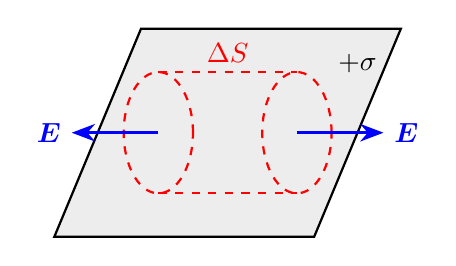
\begin{tikzpicture}[scale=1.1]
    % 带电平板 (透视效果)
    \fill[gray!20, opacity=0.7] (-2, -1.2) -- (1, -1.2) -- (2, 1.2) -- (-1, 1.2) -- cycle;
    \draw[thick] (-2, -1.2) -- (1, -1.2) -- (2, 1.2) -- (-1, 1.2) -- cycle;
    \node at (1.5, 0.8) {$+\sigma$};
    % 对称高斯圆柱体 (贯穿平面)
    \draw[dashed, red, thick] (-0.8, 0) ellipse (0.4 and 0.7);
    \draw[dashed, red, thick] (0.8, 0) ellipse (0.4 and 0.7);
    \draw[dashed, red, thick] (-0.8, 0.7) -- (0.8, 0.7);
    \draw[dashed, red, thick] (-0.8, -0.7) -- (0.8, -0.7);
    % 侧面法向和电场
    \draw[-{Stealth}, blue, very thick] (0.8, 0) -- (1.8, 0) node[right] {$\bm{E}$};
    \draw[-{Stealth}, blue, very thick] (-0.8, 0) -- (-1.8, 0) node[left] {$\bm{E}$};
    \node[red, above] at (0, 0.7) {$\Delta S$};
\end{tikzpicture}
\captionof{figure}{穿过无限大均匀带电平面的扁平高斯圆柱形曲面}
\end{center}

\textbf{解}：
由平面对称性可知，电场方向必处处垂直于带电平板，且两边离板等距离处的场强大小相等、方向相反。

作一个底面积为 $\Delta S$、两侧底面与带电板等距且平行、侧面垂直于板的圆柱形高斯面。由于侧面上 $\bm{E} \perp \mathrm{d}\bm{S}$，侧面电通量为 0；穿过两底面的电通量为：
\begin{equation*}
    \oint_S \bm{E} \cdot \mathrm{d}\bm{S} = E \Delta S + E \Delta S = 2E \Delta S
\end{equation*}
该高斯面截取板上的带电量为 $\sum q_{\text{内}} = \sigma \Delta S$。由高斯定理得：
\begin{equation*}
    2E \Delta S = \frac{\sigma \Delta S}{\varepsilon_0} \implies E = \frac{\sigma}{2\varepsilon_0}
\end{equation*}
场强分布为均匀场，方向垂直于带电板向外。
\end{example}

\subsection{静电场的环路定理与电势}

\begin{theorem}[静电场的环路定理]
静电场力是保守力，试验电荷在静电场中沿任意闭合路径移动一周，电场力所做的功恒等于零。即静电场强沿任意闭合回路的线积分为零：
\begin{equation}
    \oint_L \bm{E} \cdot \mathrm{d}\bm{l} = 0
\end{equation}
微分形式为：$\nabla \times \bm{E} = 0$。这表明静电场是无旋场，存在标量势函数。
\end{theorem}

\begin{definition}{电势与电势差}{electric_potential}
电场中某点 $P$ 的电势 $V_P$ 定义为将单位正电荷从该点经任意路径移动到选定的电势零参考点 $P_0$ 过程中电场力所做的功：
\begin{equation}
    V_P = \int_P^{P_0} \bm{E} \cdot \mathrm{d}\bm{l}
\end{equation}
两点间的电势差为：$U_{AB} = V_A - V_B = \int_A^B \bm{E} \cdot \mathrm{d}\bm{l}$。通常取无限远处为电势参考零点（当带电体分布延伸到无限远时，应选有限距离处为零参考点）。
\end{definition}

对于点电荷系，空间某点的电势满足标量叠加原理：$V = \sum_i \frac{q_i}{4\pi\varepsilon_0 r_i}$。

\subsection{电势梯度与场强关系}

\begin{theorem}[场强与电势的微分关系]
电场中任意一点的电场强度大小等于该点电势沿空间各方向变化率的最大值，方向指向电势降落最陡的方向。数学关系表述为电势梯度的负值：
\begin{equation}
    \bm{E} = -\nabla V = -\left( \frac{\partial V}{\partial x}\hat{\bm{i}} + \frac{\partial V}{\partial y}\hat{\bm{j}} + \frac{\partial V}{\partial z}\hat{\bm{k}} \right)
\end{equation}
在直角坐标系中分量式为：$E_x = -\frac{\partial V}{\partial x},\quad E_y = -\frac{\partial V}{\partial y},\quad E_z = -\frac{\partial V}{\partial z}$。
\end{theorem}

\begin{example}[由轴线电势求带电圆盘场强]
半径为 $R$、均匀带电面密度为 $\sigma$ 的薄圆盘，轴线上距离盘心 $x$ 处的电势为 $V(x) = \frac{\sigma}{2\varepsilon_0}\left(\sqrt{x^2+R^2} - x\right)$（$x>0$）。试求轴线上的电场强度。

\textbf{解}：
由轴对称性，轴线上电场沿 $x$ 轴方向，因此只需沿轴向求负导数：
\begin{align*}
    E_x = -\frac{\mathrm{d}V}{\mathrm{d}x} &= -\frac{\sigma}{2\varepsilon_0}\frac{\mathrm{d}}{\mathrm{d}x}\left(\sqrt{x^2+R^2} - x\right) \\
    &= -\frac{\sigma}{2\varepsilon_0}\left( \frac{x}{\sqrt{x^2+R^2}} - 1 \right) = \frac{\sigma}{2\varepsilon_0}\left( 1 - \frac{x}{\sqrt{x^2+R^2}} \right)
\end{align*}
当 $R \to \infty$ 时，$E_x \to \frac{\sigma}{2\varepsilon_0}$，与无限大带电平板高斯定理计算结果一致。
\end{example}


\newpage

\section{静电场中的导体和电介质}

\subsection{导体的静电平衡性质}

\begin{definition}{静电平衡状态与静电感应}{electrostatic_equilibrium}
导体内含有大量自由电子。将导体置于外电场 $\bm{E}_0$ 中时，自由电子在电场力作用下逆着电场线方向移动，使导体一端积累负电荷，另一端积累正电荷，这种现象称为\textbf{静电感应}。感应电荷建立的反向附加电场 $\bm{E}'$ 与外电场 $\bm{E}_0$ 叠加，直至导体内部合场强处处为零，内部和表面不再有自由电荷的宏观定向移动，该动态自洽调整终止的状态称为\textbf{静电平衡状态}。
\end{definition}

\begin{center}
\begin{tikzpicture}[scale=1.0]
    % 外电场线
    \foreach \y in {1.2, 0.6, 0.0, -0.6, -1.2} {
        \draw[-{Stealth}, blue!60!black, thick] (-3.6, \y) -- (-2.4, \y);
        \draw[-{Stealth}, blue!60!black, thick] (2.4, \y) -- (3.6, \y);
    }
    \node[blue!60!black, above] at (-3.0, 1.3) {外电场 $\bm{E}_0$};

    % 金属导体球
    \shade[ball color=gray!25] (0,0) circle (1.8);
    \draw[thick] (0,0) circle (1.8);

    % 感应电荷符号
    \foreach \ang in {120, 140, 160, 180, 200, 220, 240} {
        \node[blue!80!black, font=\scriptsize\bfseries] at (\ang:1.95) {$-$};
    }
    \foreach \ang in {-60, -40, -20, 0, 20, 40, 60} {
        \node[red!80!black, font=\scriptsize\bfseries] at (\ang:1.95) {$+$};
    }

    % 内部抵消过程示意
    \draw[-{Stealth}, dashed, gray!70!black, thick] (-1.0, 0.3) -- (1.0, 0.3) node[midway, above] {\footnotesize 外场 $\bm{E}_0$};
    \draw[-{Stealth}, dashed, red!70!black, thick] (1.0, -0.3) -- (-1.0, -0.3) node[midway, below] {\footnotesize 感应场 $\bm{E}'$};

    % 弯曲电场线垂直进入/引出表面
    \draw[-{Stealth}, blue!60!black, thick] (-3.2, 1.8) to[out=0, in=125] (-1.05, 1.46);
    \draw[-{Stealth}, blue!60!black, thick] (-3.2, -1.8) to[out=0, in=235] (-1.05, -1.46);
    \draw[-{Stealth}, blue!60!black, thick] (1.05, 1.46) to[out=55, in=180] (3.2, 1.8);
    \draw[-{Stealth}, blue!60!black, thick] (1.05, -1.46) to[out=-55, in=180] (3.2, -1.8);
\end{tikzpicture}
\captionof{figure}{外电场中金属导体的静电平衡与表面弯曲电力线}
\end{center}

\begin{theorem}[静电平衡的微观与宏观推论]
处于静电平衡状态的导体满足：
\begin{enumerate}
    \item 导体内部场强处处为零（$\bm{E}_{\text{内}} = 0$）；表面任一点场强方向垂直于该处表面（$\bm{E}_{\text{表}} \perp \text{表面}$）。
    \item 导体为等势体，表面为等势面（$\varphi_A = \varphi_B = \text{常数}$）。
    \item 净电荷只能分布在导体的外表面；孤立导体表面电荷面密度 $\sigma$ 与曲率成正比，尖端处电场最强易发生\textbf{尖端放电}；表面紧邻外侧场强为 $E = \frac{\sigma}{\varepsilon_0}$。
\end{enumerate}
\end{theorem}

% ------------------------- 导体例题 1 -------------------------
\begin{example}[带电导体球壳的静电平衡与电荷重新分布]
一内半径为 $R_1$、外半径为 $R_2$ 的中性金属球壳，壳内中心放一点电荷 $+q$。若将球壳外表面接地后断开，再将中心点电荷移走，求此时球壳内、外表面的带电量及空间场强分布。

\begin{center}
\begin{tikzpicture}[scale=1.1]
    % 导体球壳
    \fill[even odd rule, fill=gray!20] (0,0) circle (2.0) (0,0) circle (1.2);
    \draw[thick] (0,0) circle (1.2);
    \draw[thick] (0,0) circle (2.0);
    % 接地符号
    \draw[thick] (2.0, 0) -- (2.7, 0);
    \draw[thick] (2.7, 0.3) -- (2.7, -0.3);
    \draw[thick] (2.9, 0.2) -- (2.9, -0.2);
    \draw[thick] (3.1, 0.1) -- (3.1, -0.1);
    \node[right] at (3.1, 0) {\small 接地端};
    % 中心电荷
    \fill[red] (0,0) circle (2pt) node[below=2pt] {$+q$};
    % 感应电荷
    \foreach \ang in {30,75,120,165,210,255,300,345} {
        \node[blue, font=\tiny\bfseries] at (\ang:1.05) {$-$};
    }
    \draw[-{Stealth}] (0,0) -- (45:1.2) node[midway, above left] {\footnotesize $R_1$};
    \draw[-{Stealth}] (0,0) -- (-45:2.0) node[midway, below left] {\footnotesize $R_2$};
\end{tikzpicture}
\captionof{figure}{点电荷诱导球壳内表面感应与接地外壳屏蔽模型}
\end{center}

\textbf{解}：
\begin{enumerate}
    \item \textbf{接地阶段}：中心电荷 $+q$ 诱导内表面感应电荷 $q_{\text{内表}} = -q$。接地使球壳电势被钳制为零（$V_{\text{壳}} = 0$），外表面感应正电荷流入大地，外表面净电荷 $q_{\text{外表}} = 0$。
    \item \textbf{断开接地并移走点电荷}：断开接地后球壳总电量保持为 $Q_{\text{总}} = q_{\text{内表}} + q_{\text{外表}} = -q$。移走中心电荷后，内部不再有带电体，由高斯定理及静电平衡条件，内表面电荷转移至外表面，故最终：
    \begin{equation*}
        q_{\text{内表}} = 0, \quad q_{\text{外表}} = -q
    \end{equation*}
    \item \textbf{空间场强分布}：
    \begin{equation*}
        E(r) = \begin{cases}
            0, & r < R_2 \\
            \dfrac{q}{4\pi\varepsilon_0 r^2} \quad (\text{方向沿径向向内}), & r \ge R_2
        \end{cases}
    \end{equation*}
\end{enumerate}
\end{example}

\subsection{静电场中的电介质}

\begin{definition}{束缚电荷与电位移矢量}{dielectrics}
外电场导致各向同性电介质内部偶极子发生位移极化或转向极化，在介质表面宏观积聚不可自由移动的\textbf{束缚电荷（极化电荷）} $q'$。
为避免在静电高斯定理中直接处理难以测定的极化电荷，定义\textbf{电位移矢量} $\bm{D}$：
\begin{equation}
    \bm{D} = \varepsilon_0 \bm{E} + \bm{P} = \varepsilon_r \varepsilon_0 \bm{E} = \varepsilon \bm{E}
\end{equation}
其中 $\bm{P} = (\varepsilon_r - 1)\varepsilon_0 \bm{E}$ 为电极化强度矢量。面束缚电荷密度等于极化强度的法向分量：$\sigma' = \bm{P}\cdot\hat{\bm{n}}$。
\end{definition}

\begin{theorem}[有电介质时的高斯定理]
穿过任意闭合曲面的电位移通量，仅等于该曲面所包围的\textbf{自由电荷}代数和，介质中的束缚电荷已被吸收入 $\bm{D}$ 的定义中：
\begin{equation}
    \oint_S \bm{D} \cdot \mathrm{d}\bm{S} = \sum q_{0\text{内}}
\end{equation}
\end{theorem}

% ------------------------- 电介质例题（含三联曲线） -------------------------
\begin{example}[带电导体球外包同心电介质球壳分布曲线]
半径为 $R$ 的导体球带有自由电荷 $q$，其外包覆着厚度为 $d$、相对介电常数为 $\varepsilon_r$ 的均匀电介质层，介质外为真空。求空间各处的 $D(r)$、$E(r)$ 和电势 $V(r)$ 并绘出曲线图。

\textbf{解}：
选取同心球面为高斯面，由 $\oint \bm{D}\cdot\mathrm{d}\bm{S} = D(r) \cdot 4\pi r^2 = q_{0\text{内}}$：
\begin{enumerate}
    \item $r < R$（导体球内部）：$D = 0, \quad E = 0$。
    \item $R < r \le R+d$（介质层）：$D = \dfrac{q}{4\pi r^2}, \quad E = \dfrac{D}{\varepsilon_r \varepsilon_0} = \dfrac{q}{4\pi\varepsilon_0\varepsilon_r r^2}$。
    \item $r > R+d$（真空层）：$D = \dfrac{q}{4\pi r^2}, \quad E = \dfrac{q}{4\pi\varepsilon_0 r^2}$。
\end{enumerate}
取无穷远为零势能点，电势 $V(r) = \int_r^\infty E\,\mathrm{d}r$，分段求得：
\begin{equation*}
    V(r) = \begin{cases}
        \dfrac{q}{4\pi\varepsilon_0\varepsilon_r}\left( \dfrac{1}{R} + \dfrac{\varepsilon_r - 1}{R+d} \right), & r \le R \\[2mm]
        \dfrac{q}{4\pi\varepsilon_0\varepsilon_r}\left( \dfrac{1}{r} + \dfrac{\varepsilon_r - 1}{R+d} \right), & R < r \le R+d \\[2mm]
        \dfrac{q}{4\pi\varepsilon_0 r}, & r > R+d
    \end{cases}
\end{equation*}

\begin{center}
\begin{tikzpicture}[scale=0.96]
    % (a) D~r 曲线
    \begin{scope}[xshift=0cm]
        \draw[-{Stealth}, thick] (-0.2,0) -- (3.5,0) node[below] {$r$};
        \draw[-{Stealth}, thick] (0,-0.2) -- (0,2.6) node[left] {$D$};
        \node[below left] at (0,0) {$O$};
        \draw[dashed] (1.0, 0) node[below] {$R$} -- (1.0, 2.3);
        \draw[dashed] (2.2, 0) node[below] {\small $R+d$} -- (2.2, 2.3);
        \draw[red, very thick] (0,0) -- (1.0,0);
        \draw[red, very thick, domain=1.0:3.2, smooth] plot (\x, {1.8/(\x*\x*0.9)});
        \node at (1.6,-0.85) {\small (a) $D \sim r$ 连续衰减};
    \end{scope}

    % (b) E~r 曲线
    \begin{scope}[xshift=4.6cm]
        \draw[-{Stealth}, thick] (-0.2,0) -- (3.5,0) node[below] {$r$};
        \draw[-{Stealth}, thick] (0,-0.2) -- (0,2.6) node[left] {$E$};
        \node[below left] at (0,0) {$O$};
        \draw[dashed] (1.0, 0) node[below] {$R$} -- (1.0, 2.3);
        \draw[dashed] (2.2, 0) node[below] {\small $R+d$} -- (2.2, 2.3);
        \draw[red, very thick] (0,0) -- (1.0,0);
        \draw[red, very thick, domain=1.0:2.2, smooth] plot (\x, {1.2/(\x*\x)});
        \draw[red, very thick, domain=2.2:3.2, smooth] plot (\x, {2.6/(\x*\x)});
        \draw[dashed, red, thick] (2.2, {1.2/(2.2*2.2)}) -- (2.2, {2.6/(2.2*2.2)}); % 介质分界面的跃变
        \node at (1.6,-0.85) {\small (b) $E \sim r$ 在界面突变跃升};
    \end{scope}

    % (c) V~r 曲线
    \begin{scope}[xshift=9.2cm]
        \draw[-{Stealth}, thick] (-0.2,0) -- (3.5,0) node[below] {$r$};
        \draw[-{Stealth}, thick] (0,-0.2) -- (0,2.6) node[left] {$V$};
        \node[below left] at (0,0) {$O$};
        \draw[dashed] (1.0, 0) node[below] {$R$} -- (1.0, 2.3);
        \draw[dashed] (2.2, 0) node[below] {\small $R+d$} -- (2.2, 2.3);
        \draw[red, very thick] (0, 1.85) -- (1.0, 1.85);
        \draw[red, very thick, domain=1.0:2.2, smooth] plot (\x, {0.65 + 1.2/\x});
        \draw[red, very thick, domain=2.2:3.2, smooth] plot (\x, {2.64/\x});
        \node at (1.6,-0.85) {\small (c) $V \sim r$ 处处连续平滑连接};
    \end{scope}
\end{tikzpicture}
\captionof{figure}{含同心介质层的导体球其场变量空间分布曲线}
\end{center}
\end{example}

\subsection{电容和电容器}

\begin{definition}{电容与电容器几何结构}{capacitance}
电容 $C$ 是表征导体系统容纳电荷能力的物理量，其大小等于两导体所带等量异号电荷量 $q$ 与两极板间电势差 $U$ 的比值：
\begin{equation}
    C = \frac{q}{U} = \frac{q}{\int_{+}^{-} \bm{E}\cdot\mathrm{d}\bm{l}}
\end{equation}
电容仅由导体的形状、几何尺寸、相对间距及介质常数 $\varepsilon$ 决定。
\end{definition}

% ------------------------- 电容例题 -------------------------
\begin{example}[圆柱形电容器的电容推导]
一长为 $L$ 的同轴圆柱形电容器，内圆柱导体半径为 $R_1$，外圆柱筒内半径为 $R_2$（且 $L \gg R_2$ 略去边缘效应），其间充满相对介电常数为 $\varepsilon_r$ 的各向同性电介质。试推导该电容器的电容量。

\textbf{解}：
\begin{enumerate}
    \item 设两极板分别带有等量异号电荷 $\pm q$，轴向线电荷密度为 $\lambda = \dfrac{q}{L}$。
    \item 选取半径为 $r$、高为 $h$ 的同轴柱面为高斯面，由介质高斯定理求场强：
    \begin{equation*}
        D(r) \cdot 2\pi r h = \lambda h \implies D(r) = \frac{\lambda}{2\pi r} \implies E(r) = \frac{\lambda}{2\pi \varepsilon_r \varepsilon_0 r}
    \end{equation*}
    \item 计算极板间的电势差 $U$：
    \begin{equation*}
        U = \int_{R_1}^{R_2} E(r)\,\mathrm{d}r = \frac{\lambda}{2\pi\varepsilon_r\varepsilon_0}\int_{R_1}^{R_2} \frac{\mathrm{d}r}{r} = \frac{q}{2\pi\varepsilon_r\varepsilon_0 L}\ln\left(\frac{R_2}{R_1}\right)
    \end{equation*}
    \item 由电容定义式得：
    \begin{equation*}
        C = \frac{q}{U} = \frac{2\pi\varepsilon_r\varepsilon_0 L}{\ln(R_2 / R_1)}
    \end{equation*}
\end{enumerate}
\end{example}

\subsection{静电场的能量}

\begin{definition}{静电场能量与能量密度}{electrostatic_energy}
静电场的能量储存在空间电场中，单位体积内储存的静电能量称为\textbf{电场能量密度} $w_e$：
\begin{equation}
    w_e = \frac{1}{2}\bm{D}\cdot\bm{E} = \frac{1}{2}\varepsilon E^2 = \frac{D^2}{2\varepsilon}
\end{equation}
空间任一体积 $V$ 内的总静电能量由体积分求得：$W_e = \iiint_V w_e\,\mathrm{d}V$。
\end{definition}

% ------------------------- 能量例题 -------------------------
\begin{example}[带电球体的静电自能计算]
一半径为 $R$ 的均匀带电介质球，总电量为 $Q$。试利用电场能量体积分方法求该带电球所储存的总静电场能量 $W_e$。

\begin{center}
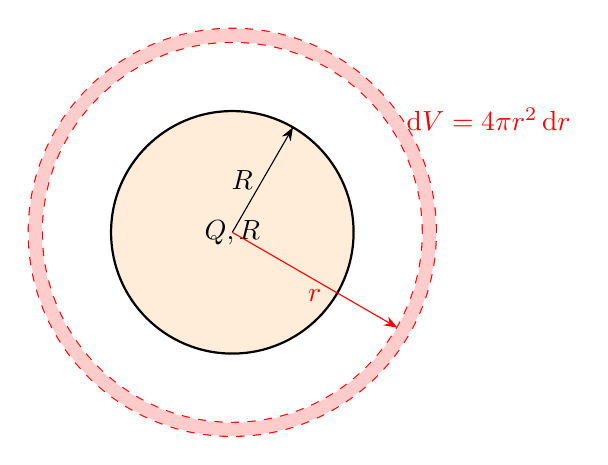
\begin{tikzpicture}[scale=1.1]
    % 球体内部
    \draw[thick, fill=orange!15] (0,0) circle (1.4);
    \node at (0, 0) {$Q, R$};
    % 薄球壳体元 dV
    \draw[dashed, red, thick] (0,0) circle (2.2);
    \draw[dashed, red, thick] (0,0) circle (2.35);
    \fill[red!20, even odd rule] (0,0) circle (2.35) (0,0) circle (2.2);
    \draw[-{Stealth}] (0,0) -- (60:1.4) node[midway, left] {$R$};
    \draw[-{Stealth}, red] (0,0) -- (-30:2.2) node[midway, below] {$r$};
    \node[red, right] at (1.9, 1.3) {$\mathrm{d}V = 4\pi r^2\,\mathrm{d}r$};
\end{tikzpicture}
\captionof{figure}{全空间薄球壳体积元划分与能量积分示意图}
\end{center}

\textbf{解}：
由高斯定理先求出真空中带电球内外的场强分布：
\begin{equation*}
    E_{\text{内}}(r) = \frac{Qr}{4\pi\varepsilon_0 R^3} \quad (r \le R), \qquad E_{\text{外}}(r) = \frac{Q}{4\pi\varepsilon_0 r^2} \quad (r > R)
\end{equation*}
取厚度为 $\mathrm{d}r$ 的同心薄球壳作为体积微元 $\mathrm{d}V = 4\pi r^2\,\mathrm{d}r$：
\begin{enumerate}
    \item 球体内部电场储存的能量：
    \begin{equation*}
        W_{\text{内}} = \int_0^R \frac{1}{2}\varepsilon_0 E_{\text{内}}^2 \cdot 4\pi r^2\,\mathrm{d}r = \frac{Q^2}{8\pi\varepsilon_0 R^6}\int_0^R r^4\,\mathrm{d}r = \frac{Q^2}{40\pi\varepsilon_0 R}
    \end{equation*}
    \item 球体外部空间储存的能量：
    \begin{equation*}
        W_{\text{外}} = \int_R^\infty \frac{1}{2}\varepsilon_0 E_{\text{外}}^2 \cdot 4\pi r^2\,\mathrm{d}r = \frac{Q^2}{8\pi\varepsilon_0}\int_R^\infty \frac{\mathrm{d}r}{r^2} = \frac{Q^2}{8\pi\varepsilon_0 R}
    \end{equation*}
    \item 全空间总静电能量为两者之和：
    \begin{equation*}
        W_e = W_{\text{内}} + W_{\text{外}} = \frac{Q^2}{40\pi\varepsilon_0 R} + \frac{Q^2}{8\pi\varepsilon_0 R} = \frac{3Q^2}{20\pi\varepsilon_0 R}
    \end{equation*}
\end{enumerate}
\end{example}

\newpage

\section{恒定磁场}

\subsection{磁感应强度与毕奥-萨伐尔定律}

\begin{definition}{磁感应强度}{magnetic_induction}
磁场对放入其中的运动电荷施加洛伦兹力，对载流导线施加安培力。引入\textbf{磁感应强度} $\bm{B}$ 描述磁场的力的性质。当电荷 $q$ 以速率 $v$ 垂直于磁场方向运动时，所受最大磁场力为 $F_{\max}$，定义：
\begin{equation}
    B = \frac{F_{\max}}{|q|v}
\end{equation}
国际单位为特斯拉（$\mathrm{T}$）。磁感应强度的方向为静止小磁针在磁场中平衡时 $N$ 极所指的方向。
\end{definition}

\begin{theorem}[毕奥-萨伐尔定律]
真空中任意电流元 $I\mathrm{d}\bm{l}$ 在距离为 $r$ 处产生的磁感应强度微元为：
\begin{equation}
    \mathrm{d}\bm{B} = \frac{\mu_0}{4\pi}\frac{I\mathrm{d}\bm{l} \times \hat{\bm{r}}}{r^2} = \frac{\mu_0}{4\pi}\frac{I\mathrm{d}\bm{l} \times \bm{r}}{r^3}
\end{equation}
其中 $\mu_0 = 4\pi \times 10^{-7}\,\mathrm{T\cdot m/A}$ 为真空磁导率。整根载流导线的合磁场满足矢量叠加原理：$\bm{B} = \int \mathrm{d}\bm{B}$。
\end{theorem}

\begin{property}[匀速运动点电荷的磁场]
电量为 $q$ 的点电荷以速度 $\bm{v}$（低速非相对论）运动时，在空间距离矢量 $\bm{r}$ 处激发的磁感应强度为：
\begin{equation}
    \bm{B} = \frac{\mu_0}{4\pi}\frac{q\bm{v} \times \hat{\bm{r}}}{r^2}
\end{equation}
若 $q>0$，$\bm{B}$ 的方向与 $\bm{v}\times\bm{r}$ 同向；若 $q<0$，则与 $\bm{v}\times\bm{r}$ 反向。
\end{property}

% ------------------------- 载流圆环例题 -------------------------
\begin{example}[载流圆线圈轴线上的磁场]
半径为 $R$ 的圆线圈通有电流 $I$。求轴线上离圆心距离为 $x$ 处的点 $P$ 的磁感应强度 $\bm{B}$。

\textbf{解}：
线圈上任意电流元 $I\mathrm{d}\bm{l}$ 与距离矢量 $\bm{r}$ 垂直，由毕奥-萨伐尔定律，产生的磁感应强度微元大小为：
\begin{equation*}
    \mathrm{d}B = \frac{\mu_0}{4\pi}\frac{I\mathrm{d}l}{r^2}
\end{equation*}
由空间对称性，垂直于轴线的分量 $\mathrm{d}B_\perp$ 积分抵消，合磁场沿轴线方向：
\begin{equation*}
    B_x = \oint \mathrm{d}B \sin\alpha = \oint \frac{\mu_0}{4\pi}\frac{I\mathrm{d}l}{R^2+x^2} \frac{R}{\sqrt{R^2+x^2}} = \frac{\mu_0 I R}{4\pi (R^2+x^2)^{3/2}} \oint \mathrm{d}l
\end{equation*}
因 $\oint \mathrm{d}l = 2\pi R$，轴线上磁感应强度为：
\begin{equation}
    B = \frac{\mu_0 I R^2}{2(R^2+x^2)^{3/2}}
\end{equation}
特别地，在圆心处（$x=0$）：$B_0 = \dfrac{\mu_0 I}{2R}$。
\end{example}

\subsection{磁场的高斯定理与安培环路定理}

\begin{theorem}[磁场的高斯定理]
通过任意闭合曲面 $S$ 的磁通量恒等于零：
\begin{equation}
    \Phi_B = \oint_S \bm{B} \cdot \mathrm{d}\bm{S} = 0 \quad (\nabla \cdot \bm{B} = 0)
\end{equation}
说明磁感应线始终是闭合无头无尾的曲线，磁场是\textbf{无源场}，不存在磁单极子。
\end{theorem}

\begin{theorem}[安培环路定理]
真空中磁感应强度 $\bm{B}$ 沿任意闭合路径 $L$ 的线积分，等于穿过以该环路为边界的任意曲面的所有传导电流代数和与 $\mu_0$ 的乘积：
\begin{equation}
    \oint_L \bm{B} \cdot \mathrm{d}\bm{l} = \mu_0 \sum_{L\text{包围}} I_i \quad (\nabla \times \bm{B} = \mu_0 \bm{j})
\end{equation}
恒定磁场是\textbf{有旋场}。
\end{theorem}

% ------------------------- 平面电流例题 -------------------------
\begin{example}[无限大均匀平面电流的磁场分布]
一无限大平面均匀流有面分布电流，线电流密度为 $j$（垂直纸面向外流出）。求平面两侧的磁感应强度。

\begin{center}
\begin{tikzpicture}[scale=1.1, >=Stealth]
    % 薄板
    \fill[green!8] (-3.8, -0.2) rectangle (3.8, 0.2);
    \draw[thick] (-3.8, 0.2) -- (3.8, 0.2);
    \draw[thick] (-3.8, -0.2) -- (3.8, -0.2);
    \draw[dashed, gray] (-4.1, 0.2) -- (-3.8, 0.2);
    \draw[dashed, gray] (-4.1, -0.2) -- (-3.8, -0.2);
    \draw[dashed, gray] (3.8, 0.2) -- (4.1, 0.2);
    \draw[dashed, gray] (3.8, -0.2) -- (4.1, -0.2);

    % 电流点阵
    \foreach \x in {-3.2, -2.4, -1.6, -0.8, 0.0, 0.8, 1.6, 2.4, 3.2} {
        \draw[red!80!black, thick] (\x, 0) circle (2.8pt);
        \fill[red!80!black] (\x, 0) circle (1.2pt);
    }
    \node[right, red!80!black, font=\small] at (4.1, 0) {线电流密度 $j\ (\odot)$};

    % 磁场 B 矢量
    \draw[->, very thick, red!85!black] (1.6, 1.55) -- (-1.6, 1.55) node[midway, above, font=\bfseries] {$\bm{B}$};
    \draw[->, very thick, red!85!black] (-1.6, -1.55) -- (1.6, -1.55) node[midway, below, font=\bfseries] {$\bm{B}$};

    % 矩形安培环路
    \draw[blue!85!black, very thick] (-1.4, -0.9) rectangle (1.4, 0.9);
    \draw[->, blue!85!black, thick] (-1.4, -0.9) -- (0.1, -0.9);
    \draw[->, blue!85!black, thick] (1.4, -0.9) -- (1.4, 0.1);
    \draw[->, blue!85!black, thick] (1.4, 0.9) -- (-0.1, 0.9);
    \draw[->, blue!85!black, thick] (-1.4, 0.9) -- (-1.4, -0.1);

    % 顶点与尺寸
    \node[below left=2pt, blue!85!black, font=\small] at (-1.4, -0.9) {$a$};
    \node[below right=2pt, blue!85!black, font=\small] at (1.4, -0.9) {$b$};
    \node[above right=2pt, blue!85!black, font=\small] at (1.4, 0.9) {$c$};
    \node[above left=2pt, blue!85!black, font=\small] at (-1.4, 0.9) {$d$};
    \draw[|<->|, thick, gray!70!black] (-1.4, -1.2) -- (1.4, -1.2) node[midway, fill=white, inner sep=2pt, font=\small] {$l$};
\end{tikzpicture}
\captionof{figure}{无限大均匀平面电流模型及闭合安培环路}
\end{center}

\textbf{解}：
由对称性分析，平面上方磁场平行于板面朝左，下方朝右，等距处 $B$ 值相等。选取矩形闭合安培环路 $abcda$（宽为 $l$），环路积分为：
\begin{equation*}
    \oint_L \bm{B} \cdot \mathrm{d}\bm{l} = \int_{ab} \bm{B}\cdot\mathrm{d}\bm{l} + \int_{bc} \bm{B}\cdot\mathrm{d}\bm{l} + \int_{cd} \bm{B}\cdot\mathrm{d}\bm{l} + \int_{da} \bm{B}\cdot\mathrm{d}\bm{l} = Bl + 0 + Bl + 0 = 2Bl
\end{equation*}
穿过环路的净电流为 $\sum I_i = jl$。由安培环路定理：
\begin{equation*}
    2Bl = \mu_0 jl \implies B = \frac{1}{2}\mu_0 j
\end{equation*}
\end{example}

\subsection{磁场中的磁介质与有介质安培环路定理}

\begin{definition}{磁介质与磁化强度}{magnetic_media}
磁介质在外磁场作用下内部产生宏观磁矩的现象称为\textbf{磁化}。定义单位体积内的分子磁矩矢量和为\textbf{磁化强度矢量} $\bm{M}$：
\begin{equation}
    \bm{M} = \lim_{\Delta V \to 0}\frac{\sum \bm{m}_i}{\Delta V}
\end{equation}
磁介质表面出现的磁化电流面密度与磁化强度的关系为：$\bm{j}_s' = \bm{M} \times \hat{\bm{e}}_n$（$\hat{\bm{e}}_n$ 为介质表面外法向）。
\end{definition}

\begin{theorem}[有磁介质时的安培环路定理]
引入辅助物理量\textbf{磁场强度} $\bm{H} = \dfrac{\bm{B}}{\mu_0} - \bm{M}$。有磁介质时的安培环路定理表述为：
\begin{equation}
    \oint_L \bm{H} \cdot \mathrm{d}\bm{l} = \sum_{L\text{包围}} I_{0\text{内}}
\end{equation}
式中右侧仅包含包围的\textbf{传导电流}（自由电流）。对于各向同性线性介质：
\begin{equation}
    \bm{B} = \mu_r \mu_0 \bm{H} = \mu \bm{H}, \quad \bm{M} = \chi_m \bm{H} = (\mu_r - 1)\bm{H}
\end{equation}
其中 $\mu_r$ 为相对磁导率，$\chi_m = \mu_r - 1$ 为磁化率。
\end{theorem}

% ------------------------- 磁介质综合大题与曲线 -------------------------
\begin{example}[长直同轴带电介质电缆的场强与磁化电流分布]
一长直圆柱导体半径为 $R_1$，其外套有内半径为 $R_1$、外半径为 $R_2$ 的同轴均匀磁介质圆筒（相对磁导率为 $\mu_2$），介质外为真空。内圆柱通过均匀分布的轴向总传导电流 $I$。求：(1) 全空间的 $H(r)$ 与 $B(r)$ 分布；(2) 磁介质内、外表面的磁化电流；(3) 绘出 $H \sim r$ 与 $B \sim r$ 曲线。

\textbf{解}：
\begin{enumerate}
    \item 选半径为 $r$ 的同轴圆形安培环路，由对称性 $\oint_L \bm{H}\cdot\mathrm{d}\bm{l} = 2\pi r H$：
    \begin{itemize}
        \item 当 $r < R_1$（内导体内，设 $\mu_1 = 1$）：包围电流 $\sum I_0 = I\dfrac{r^2}{R_1^2}$，得：
        \begin{equation*}
            H(r) = \frac{Ir}{2\pi R_1^2}, \qquad B(r) = \frac{\mu_0 Ir}{2\pi R_1^2}
        \end{equation*}
        \item 当 $R_1 < r < R_2$（磁介质层）：包围全部电流 $\sum I_0 = I$，得：
        \begin{equation*}
            H(r) = \frac{I}{2\pi r}, \qquad B(r) = \frac{\mu_0 \mu_2 I}{2\pi r}
        \end{equation*}
        \item 当 $r > R_2$（介质外真空）：包围电流仍为 $I$，得：
        \begin{equation*}
            H(r) = \frac{I}{2\pi r}, \qquad B(r) = \frac{\mu_0 I}{2\pi r}
        \end{equation*}
    \end{itemize}
    \item \textbf{磁化电流计算}：介质内磁化强度 $M(r) = (\mu_2 - 1)H(r) = \dfrac{(\mu_2 - 1)I}{2\pi r}$。
    \begin{itemize}
        \item 内表面（$r=R_1$）：面法向朝轴心，得 $j_{s1}' = M(R_1) = \dfrac{(\mu_2 - 1)I}{2\pi R_1}$，总内表面磁化电流 $I_{s1}' = j_{s1}' \cdot 2\pi R_1 = (\mu_2 - 1)I$。
        \item 外表面（$r=R_2$）：$j_{s2}' = M(R_2) = \dfrac{(\mu_2 - 1)I}{2\pi R_2}$，总外表面磁化电流 $I_{s2}' = j_{s2}' \cdot 2\pi R_2 = (\mu_2 - 1)I$。
    \end{itemize}
\end{enumerate}

\begin{center}
\begin{tikzpicture}[scale=1.0, >=Stealth]
    % (a) H ~ r 曲线
    \begin{scope}[xshift=0cm]
        \draw[->, thick] (-0.2, 0) -- (4.2, 0) node[below] {$r$};
        \draw[->, thick] (0, -0.2) -- (0, 3.0) node[left] {$H$};
        \node[below left] at (0,0) {$O$};
        
        \draw[dashed, blue!60!black] (1.5, 0) node[below, black] {$R_1$} -- (1.5, 2.2);
        \draw[dashed, blue!60!black] (2.8, 0) node[below, black] {$R_2$} -- (2.8, 1.18);
        
        % 线性上升 -> 双曲线下降 (处处连续)
        \draw[red!85!black, very thick] (0,0) -- (1.5, 2.2);
        \draw[red!85!black, very thick, domain=1.5:3.8, samples=50] plot (\x, {3.3/\x});
        
        \node[below] at (2.0, -0.7) {\small (a) $H \sim r$ 连续分布曲线};
    \end{scope}

    % (b) B ~ r 曲线 (介质界面跃升突变)
    \begin{scope}[xshift=6.5cm]
        \draw[->, thick] (-0.2, 0) -- (4.2, 0) node[below] {$r$};
        \draw[->, thick] (0, -0.2) -- (0, 3.0) node[left] {$B$};
        \node[below left] at (0,0) {$O$};
        
        \draw[dashed, blue!60!black] (1.5, 0) node[below, black] {$R_1$} -- (1.5, 2.6);
        \draw[dashed, blue!60!black] (2.8, 0) node[below, black] {$R_2$} -- (2.8, 1.4);
        
        % 内导体区
        \draw[red!85!black, very thick] (0,0) -- (1.5, 1.3);
        % 界面突变虚线 (跃升)
        \draw[red!85!black, dashed, thick] (1.5, 1.3) -- (1.5, 2.6);
        % 磁介质区 (设 mu_2 > 1)
        \draw[red!85!black, very thick, domain=1.5:2.8, samples=40] plot (\x, {3.9/\x});
        % 外界面突变下跃
        \draw[red!85!black, dashed, thick] (2.8, {3.9/2.8}) -- (2.8, {1.8/2.8});
        % 真空区
        \draw[red!85!black, very thick, domain=2.8:3.8, samples=40] plot (\x, {1.8/\x});
        
        \node[font=\footnotesize, above right] at (1.8, 2.2) {设 $\mu_2 > 1$};
        \node[below] at (2.0, -0.7) {\small (b) $B \sim r$ 在介质边界处突变};
    \end{scope}
\end{tikzpicture}
\captionof{figure}{长直载流导体外包磁介质时的 $H$ 与 $B$ 径向分布曲线}
\end{center}
\end{example}

\subsection{磁场对运动电荷与载流导线的作用}

\begin{definition}{洛伦兹力与安培力}{forces}
带电粒子 $q$ 在磁场中受到的力为\textbf{洛伦兹力}：
\begin{equation}
    \bm{F}_L = q(\bm{v} \times \bm{B})
\end{equation}
洛伦兹力垂直于速度方向，\textbf{永远不做功}。

磁场对电流元 $I\mathrm{d}\bm{l}$ 的宏观作用力为\textbf{安培力}：
\begin{equation}
    \mathrm{d}\bm{F}_A = I\mathrm{d}\bm{l} \times \bm{B} \implies \bm{F}_A = \int_L I\mathrm{d}\bm{l} \times \bm{B}
\end{equation}
\end{definition}

% ------------------------- 彻底重构优化的螺旋运动图 -------------------------
\begin{center}
\begin{tikzpicture}[scale=1.1, >=Stealth]
    % 1. 背景磁场线 (拉大间距，标在正上方空白处)
    \foreach \y in {-1.2, -0.4, 0.4, 1.2} {
        \draw[->, gray!60, thick] (-2.6, \y) -- (3.2, \y);
    }
    \node[above, gray!80!black, font=\bfseries] at (2.9, 1.25) {$\bm{B}$};

    % 2. 空间螺旋轨迹 (清晰拉伸两整周期，绝不堆叠)
    \draw[very thick, blue!80!black, domain=-2.2:1.4, samples=150, smooth] 
        plot (\x, {0.75 * sin(2.8 * (\x + 2.2) r)});

    % 3. 质点位置与速度矢量分解 (放在第一周期波峰处，极度开阔无遮挡)
    \coordinate (P) at (-1.64, 0.75);
    \fill[red!80!black] (P) circle (2.4pt);
    \node[above left=1pt, red!80!black, font=\bfseries] at (P) {$+q$};

    % 合速度 v
    \draw[->, very thick, red!85!black] (P) -- ++(32:1.4) node[above right] {$\bm{v}$};
    % 平行分量 v_parallel (沿磁场)
    \draw[->, thick, dashed, black!80] (P) -- ++(1.18, 0) node[below=2pt, font=\small] {$v_\parallel = v\cos\theta$};
    % 垂直分量 v_perp (回旋)
    \draw[->, thick, dashed, black!80] (P) -- ++(0, 0.74) node[left=2pt, font=\small] {$v_\perp = v\sin\theta$};
    
    % 夹角弧
    \draw[thin] ($(P)+(0.4,0)$) arc (0:32:0.4);
    \node at ($(P)+(0.55, 0.15)$) {\footnotesize $\theta$};

    % 4. 螺距 h 标注 (独立下移，使用干净的界线)
    \draw[gray!60, dashed] (-1.64, 0.75) -- (-1.64, -1.8);
    \draw[gray!60, dashed] (0.60, 0.75) -- (0.60, -1.8);
    \draw[|<->|, thick, black!80] (-1.64, -1.7) -- (0.60, -1.7) 
        node[midway, fill=white, inner sep=2pt, font=\small] {螺距 $h = v_\parallel T$};
\end{tikzpicture}
\captionof{figure}{带电粒子在磁场中的等距螺旋运动与速度正交分解}
\end{center}

% ------------------------- 动生电动势微元积分例题 -------------------------
\begin{example}[半圆形导线运动产生的动生电动势]
如图所示，一半径为 $R$ 的半圆形闭合导线处于磁感应强度为 $B$ 的垂直均匀磁场中，导线以速率 $v$ 沿垂直于直径 $ab$ 的方向匀速运动。求导线各段产生的动生电动势 $\mathcal{E}_{ab}$。

\begin{center}
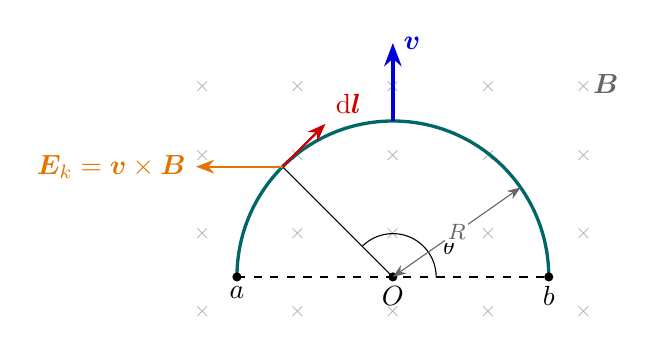
\begin{tikzpicture}[scale=1.1, >=Stealth]
    % 匀强磁场点阵 (向里)
    \foreach \x in {-2.2, -1.1, 0.0, 1.1, 2.2} {
        \foreach \y in {-0.4, 0.5, 1.4, 2.2} {
            \node[gray!60, font=\scriptsize] at (\x, \y) {$\times$};
        }
    }
    \node[above right, gray!80!black] at (2.2, 2.0) {$\bm{B}$};

    % 半圆导线
    \draw[thick, dashed] (-1.8, 0) -- (1.8, 0);
    \draw[very thick, teal!80!black] (1.8, 0) arc (0:180:1.8);
    
    % 端点与速度
    \fill (-1.8, 0) circle (1.5pt) node[below] {$a$};
    \fill (1.8, 0) circle (1.5pt) node[below] {$b$};
    \fill (0,0) circle (1.5pt) node[below] {$O$};
    \draw[->, very thick, blue!85!black] (0, 1.8) -- (0, 2.7) node[right] {$\bm{v}$};

    % 角度与微元标注
    \draw[thin] (0,0) -- (135:1.8);
    \draw[->, thick, red!80!black] (135:1.8) -- ++(45:0.7) node[above right] {$\mathrm{d}\bm{l}$};
    \draw[->, thick, orange!90!black] (135:1.8) -- ++(-1.0, 0) node[left] {$\bm{E}_k = \bm{v}\times\bm{B}$};
    \draw[thin] (0.5, 0) arc (0:135:0.5);
    \node at (0.65, 0.35) {\footnotesize $\theta$};
    \draw[<->, gray!80!black] (0,0) -- (35:1.8) node[midway, fill=white, inner sep=1pt] {\footnotesize $R$};
\end{tikzpicture}
\captionof{figure}{半圆形导线匀速切割磁力线产生的动生电动势}
\end{center}

\textbf{解}：
非静电电场（洛伦兹力场）为 $\bm{E}_k = \bm{v} \times \bm{B}$，方向水平向左。取半圆上微元 $\mathrm{d}\bm{l}$，线元大小 $\mathrm{d}l = R\mathrm{d}\theta$。
微元电动势为：
\begin{equation*}
    \mathrm{d}\mathcal{E} = (\bm{v} \times \bm{B}) \cdot \mathrm{d}\bm{l} = -v B \sin\theta \mathrm{d}l = -v B R \sin\theta \mathrm{d}\theta
\end{equation*}
沿半圆导线由 $a$ 积分至 $b$：
\begin{equation*}
    \mathcal{E}_{ab} = \int_0^\pi (-vBR\sin\theta)\,\mathrm{d}\theta = -2vBR
\end{equation*}
负号表示电动势方向由 $b$ 指向 $a$（$a$ 端电势高于 $b$ 端）。该结果等效于长度为 $2R$ 的直导线 $ba$ 切割磁力线的动生电动势。
\end{example}

\newpage

\section{电磁感应与电磁场}

\subsection{法拉第电磁感应定律与楞次定律}

\begin{definition}{电磁感应现象与磁通匝链数}{electromagnetic_induction}
当穿过闭合回路所围面积的磁通量发生变化时，回路中就会产生感应电流，这种现象称为\textbf{电磁感应现象}。
对于由 $N$ 匝线圈构成的回路，穿过各匝线圈的磁通量之和称为\textbf{磁通匝链数}（全磁通）：
\begin{equation}
    \Psi = \sum_{i=1}^{N} \Phi_{m,i} = N \Phi_m
\end{equation}
国际单位制中磁通量和全磁通的单位为韦伯（$\mathrm{Wb}$）。
\end{definition}

\begin{theorem}[法拉第电磁感应定律与楞次定律]
闭合回路中感应电动势的大小与穿过该回路的磁通量的时间变化率成正比：
\begin{equation}
    \mathcal{E}_i = -\frac{\mathrm{d}\Phi_m}{\mathrm{d}t} = -\frac{\mathrm{d}\Psi}{\mathrm{d}t}
\end{equation}
式中的负号由\textbf{楞次定律}决定：感应电流的磁场总要阻碍引起感应电流的原磁通量的变化。
\end{theorem}

\subsection{动生电动势与感生电动势}

\begin{definition}{动生电动势与非静电力}{motional_emf}
导线在磁场中运动切割磁感应线而产生的电动势称为\textbf{动生电动势}。其微观本质是运动自由电荷所受到的\textbf{洛伦兹力}：
\begin{equation}
    \mathcal{E}_m = \int_{L} (\bm{v} \times \bm{B}) \cdot \mathrm{d}\bm{l}
\end{equation}
非静电电场强度即为单位电荷所受的洛伦兹力：$\bm{E}_k = \bm{v} \times \bm{B}$。
\end{definition}

\begin{example}[转动金属棒的动生电动势]
长为 $L$ 的金属棒 $OA$ 在垂直于棒身的均匀磁场 $\bm{B}$ 中，绕端点 $O$ 在平面内以恒定角速度 $\omega$ 逆时针匀速转动。求棒上的动生电动势及各点电势高低。

\begin{center}
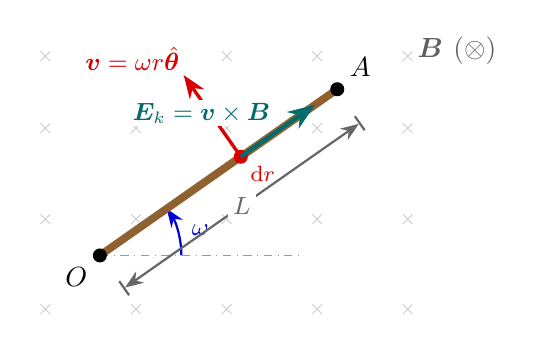
\begin{tikzpicture}[scale=1.15, >=Stealth]
    % 1. 均匀磁场向里点阵
    \foreach \x in {-0.6, 0.4, 1.4, 2.4, 3.4} {
        \foreach \y in {-0.6, 0.4, 1.4, 2.2} {
            \node[gray!45, font=\scriptsize] at (\x, \y) {$\times$};
        }
    }
    \node[above right, gray!75!black, font=\bfseries] at (3.4, 2.0) {$\bm{B}\ (\otimes)$};

    % 2. 轴心与转动棒
    \coordinate (O) at (0,0);
    \coordinate (A) at (35:3.2);
    
    \draw[dashdotted, gray!80] (O) -- (2.2, 0);
    \draw[->, thick, blue!85!black] (0.9, 0) arc (0:35:0.9);
    \node[blue!85!black, right] at (17:0.95) {\small $\omega$};

    \draw[line width=2.8pt, brown!75!black] (O) -- (A);
    \fill[black] (O) circle (2.2pt) node[below left=1pt] {$O$};
    \fill[black] (A) circle (2.2pt) node[above right=1pt] {$A$};
    
    % 3. 尺寸标注 L
    \draw[|<->|, thick, gray!80!black] ($(O)+(-55:0.45)$) -- ($(A)+(-55:0.45)$) 
        node[midway, fill=white, inner sep=2pt, font=\small] {$L$};

    % 4. 微元 dr 与矢量分解
    \coordinate (P) at (35:1.9);
    \fill[red!85!black] (P) circle (2.2pt);
    \node[below right, font=\footnotesize, red!85!black] at (P) {$\mathrm{d}r$};

    \draw[->, very thick, red!85!black] (P) -- ++(125:1.1) 
        node[above left, fill=white, inner sep=1pt, font=\small] {$\bm{v} = \omega r \hat{\bm{\theta}}$};
    \draw[->, line width=1.5pt, teal!85!black] (P) -- ++(35:1.0) 
        node[midway, above left=1pt, fill=white, inner sep=1pt, font=\small] {$\bm{E}_k = \bm{v}\times\bm{B}$};
\end{tikzpicture}
\captionof{figure}{匀强磁场中转动金属棒及其非静电场微元受力}
\end{center}

\textbf{解}：
距离转轴 $O$ 为 $r$ 处的线元 $\mathrm{d}r$，线速度大小为 $v = \omega r$。由右手定则，非静电场 $\bm{E}_k = \bm{v}\times\bm{B}$ 沿棒身由 $O$ 指向 $A$。
取微元线元矢量 $\mathrm{d}\bm{l} = \mathrm{d}r\hat{\bm{r}}$，微元电动势为：
\begin{equation*}
    \mathrm{d}\mathcal{E} = (\bm{v}\times\bm{B})\cdot\mathrm{d}\bm{l} = \omega r B\,\mathrm{d}r
\end{equation*}
沿整棒从 $O$ 积分到 $A$：
\begin{equation*}
    \mathcal{E}_{OA} = \int_0^L \omega r B\,\mathrm{d}r = \frac{1}{2}B\omega L^2
\end{equation*}
电动势方向指向端点 $A$，故端点 $A$ 电势高于中心 $O$（$V_A > V_O$）。
\end{example}

\begin{definition}{感生电场（涡旋电场）与感生电动势}{induced_electric_field}
空间随时间变化的磁场激发出一种非静电场，称为\textbf{感生电场}（或\textbf{涡旋电场}）$\bm{E}_k$。处于其中的闭合导体回路中产生的电动势称为\textbf{感生电动势}：
\begin{equation}
    \mathcal{E}_i = \oint_L \bm{E}_k \cdot \mathrm{d}\bm{l} = -\iint_S \frac{\partial \bm{B}}{\partial t}\cdot\mathrm{d}\bm{S}
\end{equation}
其微分形式为：$\nabla \times \bm{E}_k = -\frac{\partial \bm{B}}{\partial t}$。感生电场的电力线是闭合的，不是由电荷激发的，因而是无源有旋场。
\end{definition}

% ------------------------- 彻底重构的图 13 -------------------------
\begin{example}[柱状对称时变磁场的感生电场分布]
一半径为 $R$ 的长直均匀螺线管内部存在随时间线性增大的匀强磁场 $\bm{B}(t) = k t \hat{\bm{z}}$（$k > 0$ 为常数，垂直纸面向外），管外磁场近似为零。求管内及管外的感生电场分布。

\begin{center}
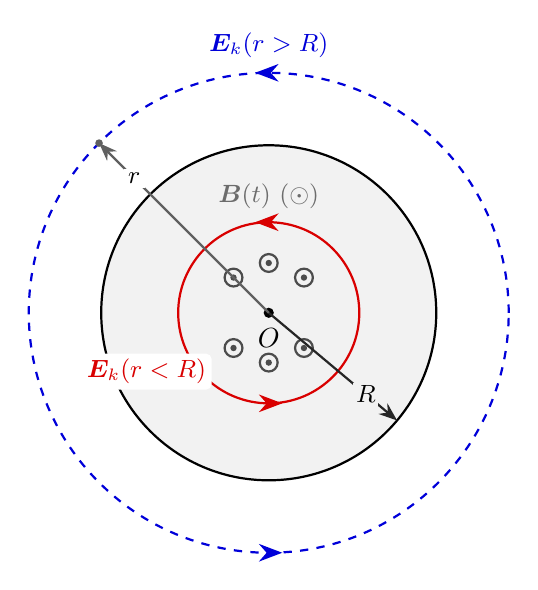
\begin{tikzpicture}[scale=1.15, >=Stealth]
    % 1. 螺线管柱面截面 (纯浅灰底，边缘清晰无任何遮挡色块)
    \fill[gray!10] (0,0) circle (1.85);
    \draw[thick] (0,0) circle (1.85);
    \fill (0,0) circle (1.6pt) node[below=2pt] {$O$};

    % 2. 磁场符号阵列与文字 (对称排布在管内上下开阔区)
    \foreach \ang in {45, 90, 135, 225, 270, 315} {
        \draw[gray!60!black, thick] (\ang:0.55) circle (2.8pt);
        \fill[gray!60!black] (\ang:0.55) circle (1.0pt);
    }
    \node[above=3pt, font=\small, gray!85!black] at (0, 0.95) {$\bm{B}(t)\ (\odot)$};

    % 3. 管内感应电场线 (r < R，红色实线圆环)
    \draw[thick, red!85!black] (0,0) circle (1.0);
    \draw[->, very thick, red!85!black] (0, 1.0) -- (-0.15, 1.0);
    \draw[->, very thick, red!85!black] (0, -1.0) -- (0.15, -1.0);
    % 文字独立放在左下方第三象限空白处，带白底防护
    \node[red!85!black, font=\small, fill=white, inner sep=2pt, rounded corners=2pt] at (-1.35, -0.65) {$\bm{E}_k (r < R)$};

    % 4. 管外感应电场线 (r > R，蓝色虚线圆环)
    \draw[thick, dashed, blue!85!black] (0,0) circle (2.65);
    \draw[->, very thick, blue!85!black] (0, 2.65) -- (-0.15, 2.65);
    \draw[->, very thick, blue!85!black] (0, -2.65) -- (0.15, -2.65);
    % 文字置于正上方最顶层
    \node[blue!85!black, font=\small, fill=white, inner sep=2pt, rounded corners=2pt] at (0, 2.95) {$\bm{E}_k (r > R)$};

    % 5. 尺寸标注线 (分离到独立象限)
    % 螺线管半径 R (第四象限 -40°)
    \draw[->, thick, black!85] (0,0) -- (-40:1.85);
    \node[fill=gray!10, inner sep=1pt, font=\small] at (-40:1.4) {$R$};
    
    % 外部观测点半径 r (第二象限 135°)
    \draw[->, thick, gray!75!black] (0,0) -- (135:2.65);
    \node[fill=white, inner sep=1.5pt, font=\small] at (135:2.1) {$r$};
    \fill[gray!75!black] (135:2.65) circle (1.2pt);
\end{tikzpicture}
\captionof{figure}{柱对称时变磁场激发的同心闭合感生电场线分布}
\end{center}

\textbf{解}：
由于磁场具有轴对称性，感生电场线呈同心圆分布，方向按楞次定律为顺时针方向。取半径为 $r$ 的同心圆环路 $L$：
\begin{equation*}
    \oint_L \bm{E}_k \cdot \mathrm{d}\bm{l} = E_k \cdot 2\pi r = -\frac{\mathrm{d}\Phi_m}{\mathrm{d}t}
\end{equation*}
\begin{enumerate}
    \item 当 $r \le R$（管内）时：穿过环路的磁通量 $\Phi_m = B \cdot \pi r^2 = k t \pi r^2$：
    \begin{equation*}
        E_k \cdot 2\pi r = k \pi r^2 \implies E_k(r) = \frac{1}{2} k r \quad (\text{线性增强})
    \end{equation*}
    \item 当 $r > R$（管外）时：磁通量仅集中在管内，$\Phi_m = B \cdot \pi R^2 = k t \pi R^2$：
    \begin{equation*}
        E_k \cdot 2\pi r = k \pi R^2 \implies E_k(r) = \frac{k R^2}{2r} \quad (\text{按 } 1/r \text{ 衰减})
    \end{equation*}
\end{enumerate}
\end{example}

\subsection{自感与互感}

\begin{definition}{自感系数与自感电动势}{self_inductance}
回路中由于自身电流发生变化而在自身回路中激发感应电动势的现象称为\textbf{自感现象}。回路的自感磁通匝链数 $\Psi_L$ 与回路电流 $I$ 成正比：
\begin{equation}
    \Psi_L = L I
\end{equation}
比例系数 $L$ 称为回路的\textbf{自感系数}（自感），单位为亨利（$\mathrm{H}$）。自身电流变化引起的自感电动势为：
\begin{equation}
    \mathcal{E}_L = -\frac{\mathrm{d}\Psi_L}{\mathrm{d}t} = -L \frac{\mathrm{d}I}{\mathrm{d}t}
\end{equation}
\end{definition}

\begin{definition}{互感系数与互感电动势}{mutual_inductance}
一个回路中的电流发生变化时，在临近另一个回路中激发出感应电动势的现象称为\textbf{互感现象}。回路 1 在回路 2 中产生的全磁通为 $\Psi_{21} = M_{21} I_1$。在无铁磁质时满足互易定理：$M_{12} = M_{21} = M$。
互感电动势分别由下式给出：
\begin{equation}
    \mathcal{E}_{21} = -M \frac{\mathrm{d}I_1}{\mathrm{d}t}, \qquad \mathcal{E}_{12} = -M \frac{\mathrm{d}I_2}{\mathrm{d}t}
\end{equation}
\end{definition}

\begin{example}[长直螺线管的自感系数计算]
长直密绕螺线管长度为 $l$，横截面积为 $S$，总匝数为 $N$。若管内充满相对磁导率为 $\mu_r$ 的介质，求该螺线管的自感系数 $L$。

\textbf{解}：
设螺线管通有电流 $I$，单位长度匝数 $n = N/l$。管内磁感应强度为匀强场：
\begin{equation*}
    B = \mu_r \mu_0 n I = \mu_r \mu_0 \frac{N}{l} I
\end{equation*}
穿过整根螺线管的全磁通（磁通匝链数）为：
\begin{equation*}
    \Psi = N \Phi_m = N (B S) = N \left( \mu_r \mu_0 \frac{N}{l} I \right) S = \frac{\mu_r \mu_0 N^2 S}{l} I
\end{equation*}
由自感定义 $\Psi = LI$，解得：
\begin{equation}
    L = \frac{\mu_r \mu_0 N^2 S}{l} = \mu_r \mu_0 n^2 V
\end{equation}
式中 $V = Sl$ 为螺线管内部体积。自感大小仅取决于线圈的几何形状、尺寸、匝数及内部介质。
\end{example}

\subsection{磁场的能量与能量密度}

\begin{definition}{载流线圈磁能与磁场能量密度}{magnetic_energy}
建立电流过程中克服自感反电动势做功所转化的能量储存在磁场中。自感为 $L$、通有电流 $I$ 的载流线圈所具有的磁场总能量为：
\begin{equation}
    W_m = \frac{1}{2} L I^2
\end{equation}
磁能分布于磁场所占据的空间中，单位体积内所储存的磁能称为\textbf{磁场能量密度} $w_m$：
\begin{equation}
    w_m = \frac{1}{2}\bm{B} \cdot \bm{H} = \frac{1}{2}\mu H^2 = \frac{B^2}{2\mu}
\end{equation}
任一体积 $V$ 内的总磁场能量由体积分求得：$W_m = \iiint_V w_m\,\mathrm{d}V$。
\end{definition}

\subsection{位移电流与麦克斯韦方程组}

\begin{definition}{位移电流与全电流安培环路定理}{displacement_current}
随时间变化的电场产生磁场的效应称为\textbf{位移电流}。麦克斯韦定义位移电流密度为电位移矢量随时间的变化率：
\begin{equation}
    \bm{j}_D = \frac{\partial \bm{D}}{\partial t} \implies I_D = \iint_S \frac{\partial \bm{D}}{\partial t} \cdot \mathrm{d}\bm{S}
\end{equation}
传导电流与位移电流统称为\textbf{全电流}，全电流是连续闭合的。拓展后的全电流安培环路定理为：
\begin{equation}
    \oint_L \bm{H} \cdot \mathrm{d}\bm{l} = \iint_S \left( \bm{j} + \frac{\partial \bm{D}}{\partial t} \right) \cdot \mathrm{d}\bm{S}
\end{equation}
\end{definition}

\begin{center}
\begin{tikzpicture}[scale=1.15, >=Stealth]
    % 1. 外部导线
    \draw[thick] (-3.4, 0) -- (-1.4, 0);
    \draw[thick] (1.4, 0) -- (3.4, 0);

    % 2. 两极板剖面
    \draw[line width=3.2pt, gray!85!black] (-1.4, -1.3) -- (-1.4, 1.3);
    \draw[line width=3.2pt, gray!85!black] (1.4, -1.3) -- (1.4, 1.3);

    % 3. 导线传导电流标注
    \draw[->, very thick, blue!85!black] (-2.9, 0.35) -- (-1.9, 0.35);
    \node[above, blue!85!black, font=\small] at (-2.4, 0.35) {$I_C$ (传导电流)};
    
    \draw[->, very thick, blue!85!black] (1.9, 0.35) -- (2.9, 0.35);
    \node[above, blue!85!black, font=\small] at (2.4, 0.35) {$I_C$};

    % 4. 极板自由电荷标注
    \node[above left, red!85!black, font=\bfseries] at (-1.4, 0.8) {$+q$};
    \node[above right, blue!85!black, font=\bfseries] at (1.4, 0.8) {$-q$};

    % 5. 极板间变化的电场线
    \foreach \y in {-0.9, -0.45, 0.45, 0.9} {
        \draw[->, thick, red!80!black] (-1.3, \y) -- (1.3, \y);
    }
    % 中轴电场线与位移电流密度公式
    \draw[->, thick, red!80!black] (-1.3, 0) -- (-0.8, 0);
    \draw[->, thick, red!80!black] (0.8, 0) -- (1.3, 0);
    \node[fill=white, inner sep=2.5pt, text=red!85!black, font=\small] at (0, 0) {$\bm{j}_D = \dfrac{\partial \bm{D}}{\partial t}$};

    % 6. 安培环路 L
    \draw[dashed, blue!85!black, thick] (0, 0) ellipse (0.5 and 1.15);
    \node[above=2pt, blue!85!black, font=\small, fill=white, inner sep=1pt] at (0, 1.15) {安培环路 $L$};
\end{tikzpicture}
\captionof{figure}{平行板电容器充放电过程中的传导电流与极板间位移电流的连续性}
\end{center}

\begin{theorem}[麦克斯韦方程组（积分形式与微分形式）]
宏观电磁场遵循的普适规律由麦克斯韦方程组统一描述：
\begin{table}[htbp]
\centering
\small
\renewcommand{\arraystretch}{1.5}
\begin{tabular}{lll}
\toprule
\textbf{基本定律} & \textbf{积分形式} & \textbf{微分形式} \\
\midrule
电场高斯定理 & $\displaystyle\oint_S \bm{D} \cdot \mathrm{d}\bm{S} = \iiint_V \rho\,\mathrm{d}V$ & $\nabla \cdot \bm{D} = \rho$ \\[3mm]
磁场高斯定理 & $\displaystyle\oint_S \bm{B} \cdot \mathrm{d}\bm{S} = 0$ & $\nabla \cdot \bm{B} = 0$ \\[3mm]
法拉第电磁感应定律 & $\displaystyle\oint_L \bm{E} \cdot \mathrm{d}\bm{l} = -\iint_S \frac{\partial \bm{B}}{\partial t}\cdot\mathrm{d}\bm{S}$ & $\nabla \times \bm{E} = -\dfrac{\partial \bm{B}}{\partial t}$ \\[3mm]
全电流安培环路定理 & $\displaystyle\oint_L \bm{H} \cdot \mathrm{d}\bm{l} = \iint_S \left(\bm{j} + \frac{\partial \bm{D}}{\partial t}\right)\cdot\mathrm{d}\bm{S}$ & $\nabla \times \bm{H} = \bm{j} + \dfrac{\partial \bm{D}}{\partial t}$ \\
\bottomrule
\end{tabular}
\end{table}
介质各向同性线性条件下的介质本构关系为：
\begin{equation}
    \bm{D} = \varepsilon \bm{E}, \qquad \bm{B} = \mu \bm{H}, \qquad \bm{j} = \sigma \bm{E}
\end{equation}
\end{theorem}

\end{document}